\icode{E-MI-MU-L4-261030-002}
（多选）
如图所示，由绝缘材料制成的内壁光滑的半圆碗固定在水平面上，\(O\) 点为圆心，带电量为 \(q_a\)、质量为 \(m_a\) 的 \(a\) 小球固定在半圆碗底端的 \(A\) 点，带电量为 \(q_b\)、质量为 \(m_b\) 的 \(b\) 小球静止于半圆碗内的 \(B\) 点，此时 \(\angle AOB =\) \,\qty{74}{\degree}。由于 \(a\)、\(b\) 两小球的质量变化或电荷量变化使得 \(b\) 小球沿半圆碗的内壁缓慢下滑，恰好静止于 \(C\) 点，\(\angle AOC =\) \,\qty{60}{\degree}，此时 \(a\)、\(b\) 两小球的质量分别为 \(m^\prime_a\)、\(m^\prime_b\)，电荷量分别为 \(q_a^\prime\)、\(q^\prime_b\)，已知 \(a\)、\(b\) 两小球均可视为点电荷，\(\sin\)\qty{37}{\degree}=0.6，\(\cos\)\qty{37}{\degree}=0.8，则下列说法正确的是\paren[]

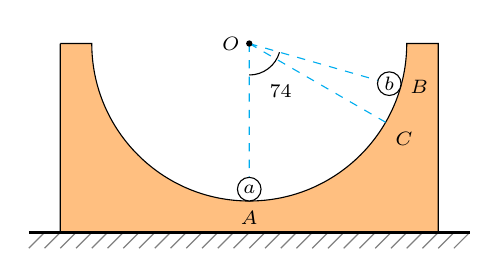
\begin{tikzpicture}[font=\scriptsize]
	\draw[fill=orange!50] (-2.4,0)--(-2,0) arc(-180:0:2)--(2.4,0)--(2.4,-2.4)--(-2.4,-2.4)--(-2.4,0);
	\draw[dashed,cyan] (0,0)coordinate(o)--(-90:2) (o)--(-30:2) (o)--(-16:2);
	\draw[fill=white] (-90:1.85)node{ \(a\)} circle(.15) (-16:1.85)node{ \(b\)} circle(.15);
	\fill (o)node[left]{ \(O\)} circle(.04);
	\draw (0,-.4) arc(-90:-16:.4);
	\node at(0,-2)[below]{ \(A\)};
	\node at(-16:2)[right]{ \(B\)};
	\node at(-30:2)[below right]{ \(C\)};
	\node at(.4,-.6){\qty{74}{\degree}};
	\foreach \x in {-2.8,-2.6,...,2.6}
		\draw[gray] (\x,-2.6)--++(.2,.2);
	\draw[thick] (-2.8,-2.4)--(2.8,-2.4);
\end{tikzpicture}
\begin{choices}
	\item \(b\) 小球受到的支持力一定大于其重力
	\item \(b\) 小球的质量和电荷量至少有一个应发生变化
	\item 可能仅是 \(b\) 小球的质量 \(m_b^\prime\) 增加至 \(\frac{216}{125}m_b\)
	\item 可能仅是 \(a\)、\(b\) 两小球电荷量的乘积 \(q_a^\prime q_b^\prime\) 减小至 \(\frac{5}{6}q_a q_b\)
\end{choices}
\begin{answer}
    BC\qquad 提示：如图所示，受力分析可知\(N = m_b g\)，\(F = k \frac{q_a q_b}{(2r\sin(\frac{\theta}{2}))^2} = 2 m_b g\sin(\frac{\theta}{2})\)，\(\frac{q_a q_b}{m_b} = \frac{8gr^2}{k}[\sin(\frac{\theta}{2})]^3\)

\begin{tikzpicture}[>=stealth,font=\scriptsize]
	\draw[fill=orange!30] (-2.4,0)--(-2,0) arc(-180:0:2)--(2.4,0)--(2.4,-2.4)--(-2.4,-2.4)--(-2.4,0);
	\draw[dashed,cyan!50] (0,0)coordinate(o)--(-90:2) (o)--(-16:2) (-90:1.85)--(-16:1.85);
	\draw[fill=white,draw=gray] (-90:1.85)circle(.15) (-16:1.85) circle(.15);
	\fill (o)node[left,gray]{ \(O\)} circle(.04);
	\draw[gray] (0,-.4) arc(-90:-16:.4);
	\node at(.4,-.6)[gray]{\(\theta\)};
	\foreach \x in {-2.8,-2.6,...,2.6}
		\draw[gray!50] (\x,-2.6)--++(.2,.2);
	\draw[thick,gray] (-2.8,-2.4)--(2.8,-2.4);
	\draw[->] (-16:1.85)coordinate(g)--++(0,-1.6)node[below]{\(mg\)};
	\draw[->,magenta] (g)--++(164:1.6)node[above]{\(N\)};
	\draw[->,teal] (g)--++(37:{3.2*sin(37)})node[right]{\(F\)};
	\draw[dashed,magenta] (g)--++(-16:1.6);
	\draw[dashed,teal] ($(g)+(0,-1.6)$)--++(37:{3.2*sin(37)});
	\draw[dashed,cyan] (g)--++(-53:{1.6*cos(37)});
\end{tikzpicture}
\end{answer}